%_______________________________________________________________________________
%class
%_______________________________________________________________________________
%\documentclass[a4paper,11pt,onecolumn,final,german,openbib]{scrbook}
\documentclass[a4paper,11pt,twosided,final,german,openbib,pdftex,listof=totoc,bibliography=totoc]{scrbook}
%_______________________________________________________________________________
% page borders
%_______________________________________________________________________________
\addtolength{\headheight}{2cm}
%\addtolength{\topmargin}{2cm}
\setlength{\oddsidemargin}{1.0cm}
\setlength{\evensidemargin}{0.5cm}
\setlength{\textwidth}{14.3cm}
\setlength{\parindent}{0mm}

%_______________________________________________________________________________
% packages
%_______________________________________________________________________________
\usepackage[english]{babel}
\usepackage{amsmath, amssymb}
\usepackage[utf8]{inputenc}
\usepackage{graphicx}
\usepackage{enumerate}
\usepackage{multirow}
\usepackage{subfigure}
\usepackage{dsfont}
\usepackage{slashed}
\usepackage{textcomp}
\usepackage{url}
\usepackage{amsmath}
\usepackage{hyperref}

\usepackage{wrapfig}
\usepackage{nicefrac}
\usepackage[backend=bibtex,style=numeric]{biblatex}
\usepackage{lmodern}
\usepackage{epigraph}
\usepackage[T1]{fontenc}
\usepackage{yfonts,color}
\usepackage{titlesec}
\usepackage{lettrine}
\usepackage{fancyhdr}
\usepackage[compat=1.0.0]{tikz-feynman}
\usepackage{tikz}
\usetikzlibrary{decorations.pathmorphing,decorations.markings,trees}




\pagestyle{fancy}
\tikzset{
	particle/.style={thick,draw=blue, postaction={decorate},
		decoration={markings,mark=at position .5 with {\arrow[blue]{triangle 45}}}},
	gluon/.style={decorate, draw=black,
		decoration={coil,aspect=0}}
}

\widowpenalty10000
\clubpenalty10000






\titleformat{\chapter}[block]
{\Large\bfseries}
{\raisebox{-\height}{\sffamily\scriptsize\MakeUppercase{\chaptertitlename}}%
	\space\raisebox{-\height}{\bigchapternumber}\space}
{0pt}
{\printtitle}

\newlength\pretitlewidth
\newcommand\bigchapternumber{\resizebox{24pt}{!}{\mdseries\thechapter}}
\newcommand{\printtitle}[1]{%
	\settowidth{\pretitlewidth}{%
		{\sffamily\scriptsize\MakeUppercase{\chaptertitlename}}\space
		{\bigchapternumber}\space
	}%
	\parbox[t]{\dimexpr.8\textwidth-\pretitlewidth}{%
		\linespread{1.5}\selectfont
		\hrule depth 1pt
		\vspace{3ex}
		\raggedright\bfseries #1
	}%
}




\addbibresource{Masterarbeit_Martin_Sobotzik.bib}
%_______________________________________________________________________________
% bold fonts for headings
%_______________________________________________________________________________
\font\afont=cmssbx10 scaled \magstep5     % for the title
\font\bfont=cmssbx10 scaled \magstep4     % for chapter headings
\font\cfont=cmssbx10 scaled \magstep3
\font\dfont=cmssbx10 scaled \magstep2     % for section headings and author name
%\font\efont=cmssbx10 scaled \magstephalf

%_______________________________________________________________________________
% index depth
%_______________________________________________________________________________
\setcounter{secnumdepth}{3}
\setcounter{tocdepth}{3}

%_______________________________________________________________________________
% new commands
%_______________________________________________________________________________
\newcommand{\demi}{\frac{1}{2}}

%_______________________________________________________________________________
% renewed commands
%_______________________________________________________________________________
% \renewcommand{\topfraction}{1.}       % this is important for figure placement
% \renewcommand{\bottomfraction}{1.}
\makeatletter
\renewcommand\paragraph{\@startsection{paragraph}{4}{\z@}%
  {-3.25ex\@plus -1ex \@minus -.2ex}%
  {1.5ex \@plus .2ex}%
  {\normalfont\normalsize\bfseries}
}
\makeatother

%_______________________________________________________________________________
% special words, hyphenation
%_______________________________________________________________________________
\hyphenation{Ba-che-lor-ar-beit}









\pagestyle{fancy}






\pagestyle{headings}
%for changing the style on a specific page use \thispagestyle{e.g., empty}

%_______________________________________________________________________________
%_______________________________________________________________________________
\begin{document}
\pagenumbering{roman}

%_______________________________________________________________________________
\begin{titlepage}
  \vspace*{6mm}
  \begin{center}
     {\afont Systematic Studies on Reconstruction Efficiency at Belle II}
     \\[3.5cm]
     {\large von}
     \\[3.5cm]
     {\dfont Martin Sobotzik}
     \\[2cm]
     {\large Masterarbeit in Physik \/\\
        vorgelegt dem Fachbereich Physik, Mathematik und Informatik (FB 08) \/\\
        der Johannes Gutenberg-Universit\"at Mainz \/\\
        am 3. Dezember 2019}
   \end{center}
   \vfill
   1. Gutachter: Prof. Dr. Wolfgang Gradl\\	
   2. Gutachter: Prof. Dr. Habe D\"unkel \\
   \vfill

\end{titlepage}
\newpage 
 

\thispagestyle{empty}
Ich versichere, dass ich die Arbeit selbstst\"andig verfasst und keine 
anderen als die angegebenen Quellen und Hilfsmittel benutzt sowie 
Zitate kenntlich gemacht habe.
\\
\\[3.5cm] 
Mainz, den [Datum] [Unterschrift]
\vfill
\noindent 
Martin Sobotzik\\
Institut f\"ur Kernphysik\\
Johannes-Joachim-Becher-Weg 45\\
Johannes Gutenberg-Universit\"at
D-55128 Mainz\\
{\href{msobotzi@students.uni-mainz.de}{msobotzi@students.uni-mainz.de}}

%_______________________________________________________________________________





\newpage

\epigraph{In der Mathematik versteht man die Dinge nicht. Man gew\"ohnt sich nur an sie.}{John von Neumann}






















\renewcommand\contentsname{Contents}
\renewcommand\figurename{Figure}
\renewcommand\tablename{Table}
\tableofcontents
\clearpage

\mainmatter
\sloppy

%_______________________________________________________________________________
\chapter{Introduction}
\label{sec:Introduction}

{\em Dieses Dokument richtet sich an Studierende am Fachbereich 08 im 
Studiengang Bachelor of Science (Physik). Sie finden hier Beispiele 
f\"ur eine m\"ogliche Gliederung Ihrer Arbeit und Hinweise zur 
Strukturierung des Inhalts. Selbstverst\"andlich sollen Sie diese 
Gliederung nach den Gegebenheiten Ihrer Bachelorarbeit anpassen. 
Besprechen Sie rechtzeitig mit Ihrem Betreuer, ob Ihr Entwurf sinnvoll 
ist. Holen Sie sich auch Anregungen zur Gestaltung von Abschlussarbeiten 
aus der Literatur ().
\medskip

Sofern Sie sich dazu entscheiden, Ihr Dokument in \LaTeX\ zu erstellen, 
k\"onnen Sie diese Datei als Vorlage verwenden. Fast die gesamte 
Literatur in der Physik verwendet \LaTeX, vor allem wegen der 
ausgezeichneten M\"oglichkeiten f\"ur das Formelschreiben.
}
\bigskip

In der Einleitung Ihrer Bachelorarbeit sollte das Thema der Arbeit 
m\"oglichst allgemeinverst\"andlich eingef\"uhrt werden. Gehen Sie 
dabei auch auf das weitere Umfeld der Arbeit ein und erl\"autern Sie, 
warum Aufgabenstellung und Herangehensweise interessant sind. Auch 
die weitere Gliederung kann angesprochen werden, um dem Leser einen 
ersten \"Uberblick \"uber den nachfolgenden Text zu geben.

\chapter{Standard Model}
\label{cha:SM}

\lettrine[lines=3]{T}{he} standard model of particle physics (SM) is a theory that describes three of the four fundamental known forces in the universe: the electromagnetic, the weak and the strong force. 

 At the current level of experimental precision and the reached energies so far, it is the best theory describing these forces.
 
 Unfortunately the standard model fails to explain a variety of different observations and since gravitation is not included in the standard model, it is easy to see that the standard model is not complete.
 
\section{The Standard Model}
\label{sec:SM}

The standard model is based on the idea that matter is made of particles with no internal structure. These particles can interact with each other by exchanging other particles which are associated to the fundamental forces. The standard model includes the \textit{quantum electrodynamic} (QED), the \textit{electroweak theory} (EWT) and the \textit{quantum chromodynamic} (QCD) as well as the \textit{Higgs mechanism}.

The QED describes all phenomenons caused by photons ($\gamma$) and charged point-like particles like electron and positrons. In the 1920s Paul Dirac laid the foundation for the QED while computing the coefficient of spontaneous emission of an atom. The description of the weak force (\textit{quantum flavordynamics}, QFD) and the QED got merged by Sheldon Glashow in the early 1960s. The exchange particles of the weak force are the $Z$ and $W^{\pm}$ \textit{bosons}. A few years later, Steven Weinberg and Abdus Salam independently proposed a theory that included the \textit{Higgs mechanism} whereby the \textit{electroweak theory} (EQT) emerged. The \textit{Higgs mechanism} is the reason why the \textit{gauge bosons} have mass.
Finally the standard model reached its modern form after combining the EWT and the theory of the strong interaction (\textit{quantum chromodynamic}, QCD). This was done by Abraham Pais and Sam Treiman in 1975. The exchange particles for the strong force are the \textit{gluons} ($g$). They >>\textit{glue}<< quarks together, forming \textit{hadrons} like \textit{mesons} (even number of quarks) and \textit{baryons} (odd number of quarks). \cite{RiseStandard}
\newline  

\begin{figure}[h!]
	\centering
	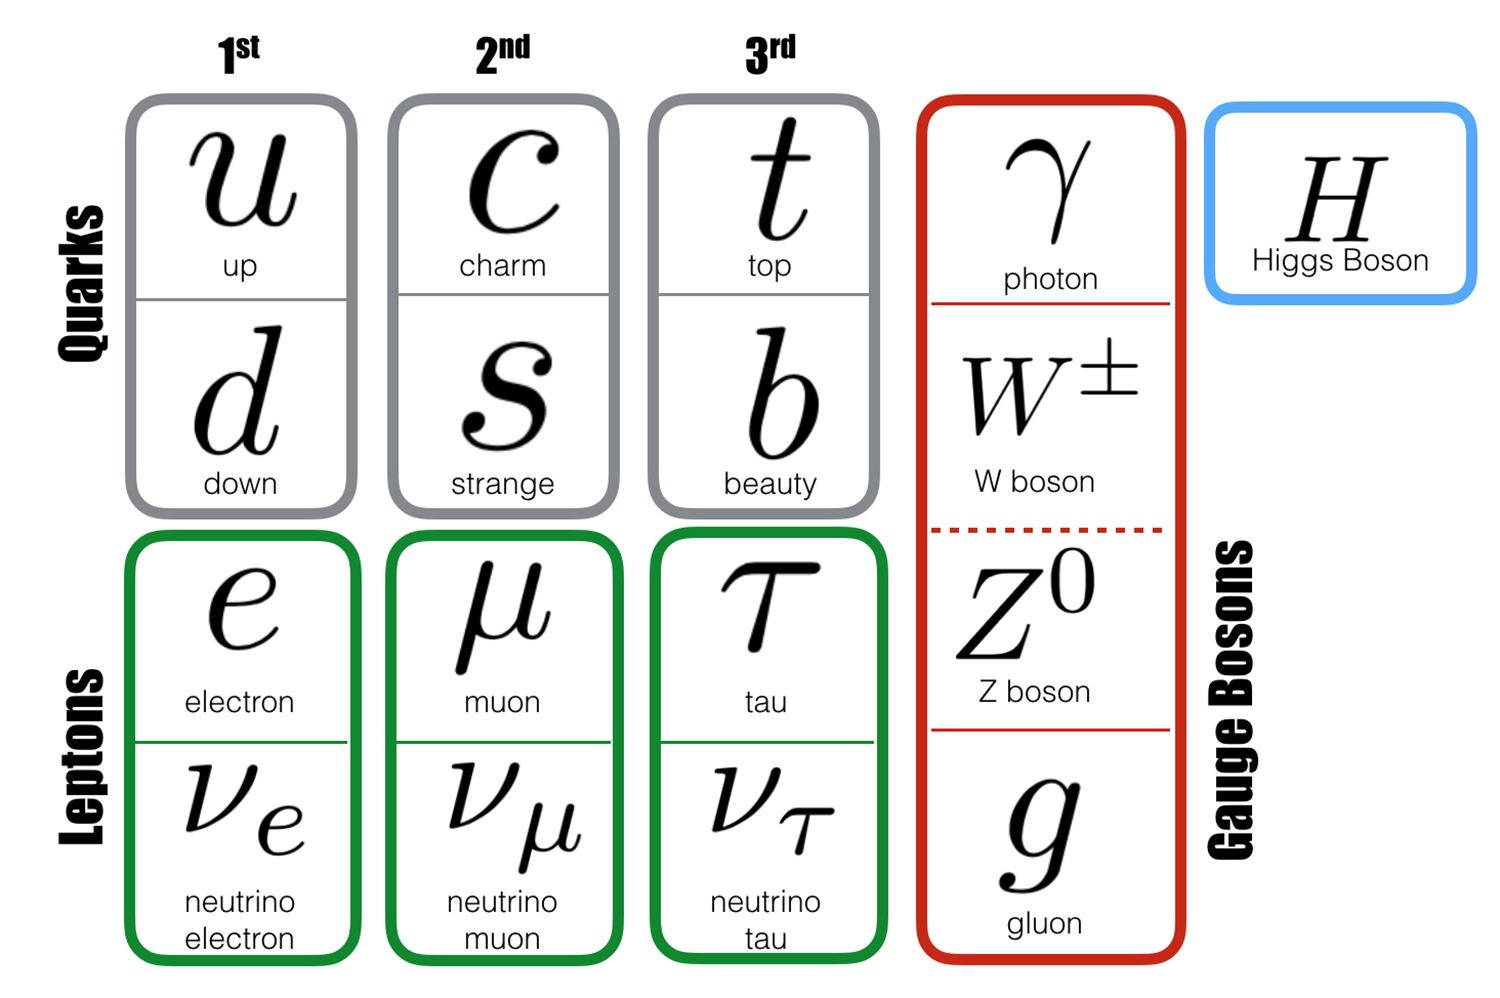
\includegraphics[width=15cm]{Bilder/SM.png}
	\caption[Standard Model]{The particles of the Standard Model include three families of quarks and leptons, four gauge bosons and the Higgs boson. The beige background indicates which bosons interact with which fermions. \cite{SMFigure}}
	\label{fig:SM}
\end{figure}



Figure \ref{fig:SM} shows the fundamental particles of the standard model. It includes three families of quarks and leptons so-called \textit{fermions}, four \textit{gauge bosons} and the Higgs \textit{boson}. Fermions and bosons differ by the spin. Spin is a degree of freedom, which had to be introduced to conserve the angular momentum in the Dirac equation. The matter forming fermions have a half-integral spin (in units of the reduced Planck constant $\hbar$) and the bosons (the exchange particles as well as the Higgs particle) have an integer spin. The fermion family can be sectioned into two families. The \text{quark} and the \textit{lepton} family. 
The quark familiy consist of up- (u), down- (d), strange- (s), charm- (c), bottom- (b) and top- (t) quark. Quarks have fractional electric charge values. u-, c- and t-quark have an electric charge of $\nicefrac{2}{3} \,e$ and d-, s- and b-quark have an electric charge of $-\nicefrac{1}{3} \,e$. As indicated in figure \ref{fig:SM} by the beige background, quarks can interact with all four gauge bosons.
The lepton family is made of the electron ($e$), the muon ($\mu$) and the tau ($\tau$) and their corresponding neutrinos $\nu_e,\nu_{\mu} \textrm{ and } \nu_{\tau}$. The neutrinos can only interact with the weak exchange particles ($W^{\pm}$ and $Z$ bosons). Since the electrons, muons and taus are charged, they can also interact with photons ($\gamma$).

All fermions also have so-called \textit{antiparticles}. Antiparticle have the same mass as their corresponding particle but they have opposite charge. For example, the antiparticle of the electron is the positron. Both have the same mass and the same spin but the electron has an electric charge of $-1\,e$ and the positron has an electric charge of $+1\,e$.
When a particle collides with its antiparticle annihilation can occur. In an annihilation process the incoming particles are destroyed to produce other particles. The total energy and momentum of the initial pairs is conserved. 
\newline 


All visible matter in the universe is made of fermions from the first family. For example, atoms consist of protons and neutrons, each of which is a combination of up and down quarks. In the electron shell of an atom the eponymous electrons are located. Pauli proposed the neutrino in the 1930 to explain the energy spectrum of electrons in $\beta$-decays. Since neutrinos are only weak interacting particles, they were not observed until 1956.\cite{REINES19941} With increasing energy, the second and third family have been gradually discovered, first from cosmic ray experiments in the 1930s up to the discovery of the Higgs boson at the LHC in 2012. Parallel to the experimental discoveries, the theory also evolved, partially explaining the results and in part motivating new experiments through predictions.
\newline

\section{Physics Beyond The Standard Model}

Despite the success of the standard model as an effective theory, it fails answering a lot of open questions. As already mentioned, the standard model only includes three out of four fundamental forces. It does not include gravity, therefore, the standard model is not valid at energy scales approaching the Planck energy $E_P \approx 1.22\cdot 10^{19}\,\textrm{GeV} $.\cite{sivaram2007special} It is also unable to explain dark matter, dark energy and the matter/antimatter asymmetry in the universe which is directly linked to charged-parity violation.\cite{HAMBYE2012193}

\section{Bhabha Scattering}
\label{sec:Bhabha}


\tikzset{
	photon/.style={decorate, decoration={snake}, draw=red},
	electron/.style={draw=blue, postaction={decorate},
		decoration={markings,mark=at position .55 with {\arrow[draw=blue]{>}}}},
	gluon/.style={decorate, draw=magenta,
		decoration={coil,amplitude=4pt, segment length=5pt}} 
}



\tikzset{
	photon/.style={decorate, decoration={snake}, draw=red},
	particle/.style={draw=blue, postaction={decorate},
		decoration={markings,mark=at position .5 with {\arrow[draw=blue]{>}}}},
	antiparticle/.style={draw=blue, postaction={decorate},
		decoration={markings,mark=at position .5 with {\arrow[draw=blue]{<}}}},
	gluon/.style={decorate, draw=black,
		decoration={coil,amplitude=4pt, segment length=5pt}}
}






\begin{tikzpicture}[
thick,
% Set the overall layout of the tree
level/.style={level distance=1.5cm},
level 2/.style={sibling distance=2.6cm},
level 3/.style={sibling distance=2cm}
]
\coordinate
child[grow=left]{
	child {
		node {$e^+$}
		% The 'edge from parent' is actually not needed because it is
		% implicitly added.
		edge from parent [particle]
	}
	child {
		node {$e^-$}
		edge from parent [antiparticle]
	}
	edge from parent [photon] node [above=3pt] {$\gamma$}
}
% I have to insert a dummy child to get the tree to grow
% correctly to the right.
child[grow=right, level distance=0pt] {
	child {
	node {$e^-$}
	% The 'edge from parent' is actually not needed because it is
	% implicitly added.
	edge from parent [particle]
}
child {
	node {$e^+$}
	edge from parent [antiparticle]
}
edge from parent [photon] 
}
	
;
\end{tikzpicture}

\begin{tikzpicture}[
thick,
% Set the overall layout of the tree
level/.style={level distance=1.5cm},
level 2/.style={sibling distance=2.6cm},
level 3/.style={sibling distance=2cm}
]
\coordinate
child[grow=up]{
	child {
		node {$e^+$}
		% The 'edge from parent' is actually not needed because it is
		% implicitly added.
		edge from parent [antiparticle]
	}
	child {
		node {$e^+$}
		edge from parent [particle]
	}
	edge from parent [photon] node [right=3pt] {$\gamma$}
}
% I have to insert a dummy child to get the tree to grow
% correctly to the right.
child[grow=down, level distance=0pt] {
	child {
		node {$e^-$}
		% The 'edge from parent' is actually not needed because it is
		% implicitly added.
		edge from parent [antiparticle]
	}
	child {
		node {$e^-$}
		edge from parent [particle]
	}
	edge from parent [photon] 
}

;
\end{tikzpicture}








%_______________________________________________________________________________
\chapter{Experimental Setup at SuperKEKB}
\label{sec:SetupKEK}

\lettrine[lines=3]{S}{uperKEKB} is an two-ring, asymmetric\footnote{asymmetric means that there is an energy difference between the two colliding beams}, electron positron accelerator, which is located at KEK (\textit{High Energy Accelerator Research Organization}) in Tsukuba Japan. 
The electron beam has an energy of $7\,\textnormal{GeV}$ 
and the positron beam has an energy of $4\,\textnormal{GeV}$. These beams collide with a center-of-momentum energy of about $10.58\,\textnormal{GeV}$, which is close to the mass of the $\Upsilon(4\textnormal{S})$ resonance. Therefore SuperKEKB is a so-called \textit{B-factory}. The decay products are then detected by the  Belle II detector to study the properties of these B mesons with high precision. In early 2018 Belle II started taking data. One goal of Belle II is to study CP-Violation with respect to new physics.\cite{B2B}

\section{KEKB and SuperKEKB}
\label{sec:KEK}
This section will only provide a rough overview of the SuperKEKB accelerator since the focus of this work is on the analysis. 

SuperKEKB is an upgrade of the KEKB accelerator. KEKB was also an asymmetric electron positron accelerator in the period from 1998 to 2010, but the energies were different compared to SuperKEKB. At KEKB the electrons were accelerated to an energy of $8\,\textrm{GeV}$ and the positrons to an energy of $3.5\,\textrm{GeV}$. KEKB was also a B-factory and the reaction products were then detected in the Belle detector. In 2009 KEKB achieved an instantaneous luminosity of $2.11 \cdot 10^{34}\,\textrm{cm}^{-1}\textrm{s}^{-1}$. This was the world record at that time. KEKB was discontinued after more than 10 years, to be upgraded to SuperKEKB.\cite{PTEP}


\begin{figure}[h!]
\begin{center}
	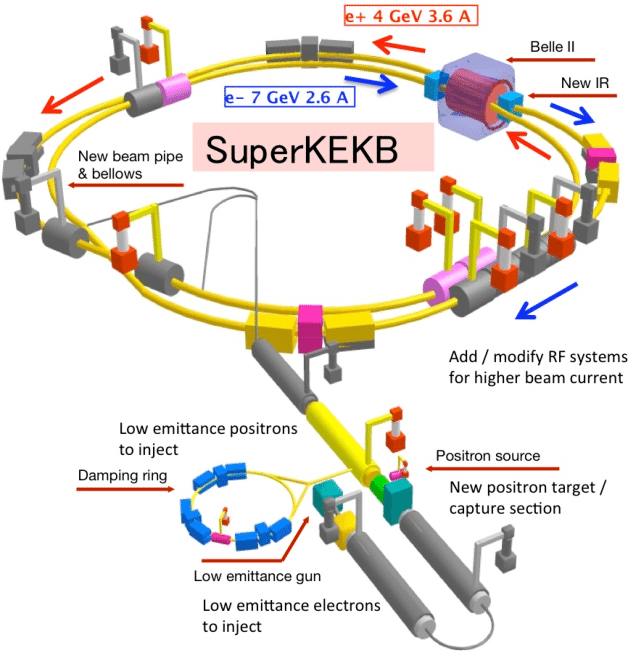
\includegraphics[width=8cm]{Bilder/SuperKEKB.png}
	
	\caption[SuperKEKB Collider]{The SuperKEKB collider.\cite{SKEKAcc}}
	\label{fig:SuperKEKB}
\end{center}
\end{figure}

In figure \ref{fig:SuperKEKB} you can see the schematic layout of the SuperKEKB accelerator. The electrons are start at the Low emittance gun. They are then accelerated in the \textit{J}-shaped linear particle accelerator (linac). Due to lack of space, the linac has to have this special form.\cite{KEKBJArc} After the curve and a second acceleration stage the electrons hit the positron production target, where the positrons are created. After this target there are more acceleration stages, before the two beam are then injected into their independent storage rings. The electrons are stored in the high-energy ring (HER) and the positrons are stored in the low-energy ring (LER). Each of these rings has a circumference of about $3\,\textrm{km}$. Both beams collide at the interaction region (IR). The products of the collisions are then detected by the Belle II detector, an upgraded version of the Belle detector.\cite{B2B} (See chapter \ref{sec:BelleII})

SuperKEKB uses a smaller asymmetry in the beam energies compared to KEKB. This allows the usage for higher beam currents and better focusing magnets. This can then result into a higher luminosity. The goal is to achieve a 40 times higher luminosity with SuperKEKB compared to KEKB.
An integrated luminosity of $50\,\textrm{ab}^{-1}$ will be achieved by 2025.\cite{B2B}

The instantaneous luminosity $\mathcal{L}$ specifies the performance of the collider. Knowing $\mathcal{L} $ and the cross section $\sigma$ one can calculate the events per second for a process by the following formula.
\begin{equation}
\frac{\textrm{d}N}{\textrm{d}t} = \mathcal{L} \cdot \sigma
\end{equation} 

To increase the event rate one has to increase the instantaneous luminosity since $\sigma$ is given by the processes. The instantaneous luminosity can be calculate by
\begin{equation}
	\mathcal{L} = \frac{N_{e^-}N_{e^+}f_c}{4\pi \sigma_x \sigma_y} \cdot S
	\label{eq:Lumi}
\end{equation}
 assuming that both beams have a Gaussian profile of horizontal and vertical size $\sigma_x$ and $\sigma_y$. In equation \ref{eq:Lumi} $N_{e^-}$ is the number of particles in an electron bunch and $N_{e^+}$ is the number of particles in a positron bunch. $f_c$ is the average crossing rate, which can be calculated by $f_c = n \cdot f_r$. Where $n$ is the number of bunches and $f_r$ is the revolution frequency. $S$ is a reduction factor which takes geometrical effects linked to the finite cross section and bunch length into account.\cite{herr2006concept} SuperKEKB increased the luminosity by a factor of two compared to KEKB by increasing the number of bunches and the number of particles per bunch.
 
\begin{figure}[h!]
	\centering
	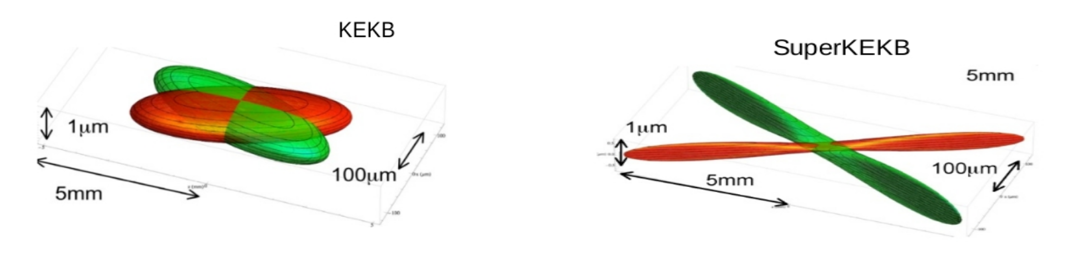
\includegraphics[width=14.5cm]{Bilder/bsSKEK}
	
	\caption[Sketch of the Beam Crossing for KEKB and SuperKEKB]{Sketch of the beam crossing at KEKB (left) and SuperKEKB (right). At KEKB the size of the interaction region was about $10\,\textrm{mm}$. At SuperKEKB it is about $0.5\,\textrm{mm}$}
	\label{fig:beamsize}
\end{figure}

Also the size of the interaction region at SuperKEKB is just one twentieth of what it was at KEKB, resulting in a vertical beam size of $\sigma \approx 50\,\textrm{nm} $. This can be seen in figure \ref{fig:beamsize}. This decrease in beam size, along with the increase in the beam currents, it results in a overall 40-fold increase in luminosity.  \cite{B2TR} \cite{B2B}



\section{The Belle II Detector}
\label{sec:BelleII}

The Belle II detector is an upgraded version of the Belle detector which was a solid-angle magnetic spectrometer located at the interaction region of KEK. In figure  \ref{fig:Belle2} a sketch of the Belle II detector is shown. The detector contains of a variety of sub-detectors, each fulfilling a specific purpose.
 
\begin{figure}[h!]
	\centering
	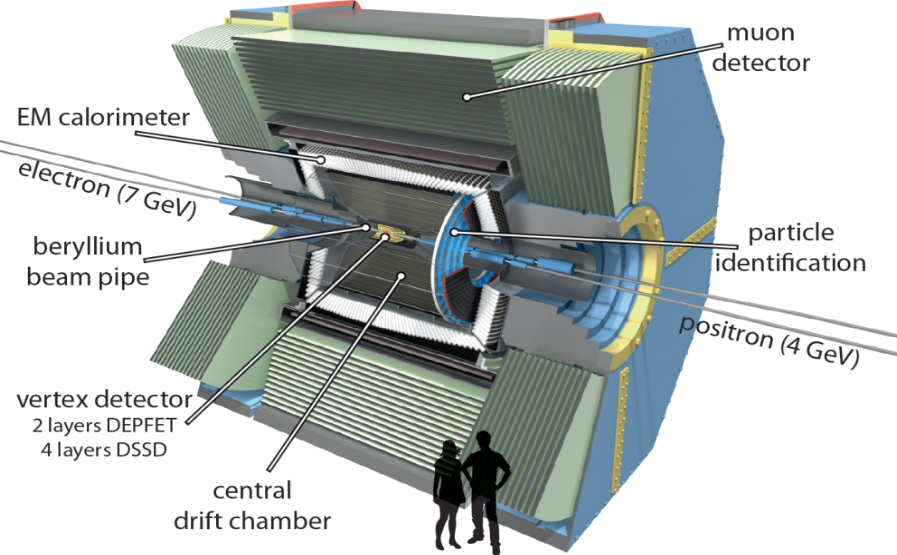
\includegraphics[width=12.5cm]{Bilder/Belle2.png}
	
	\caption[Belle II Detector]{Schematic view of the Belle II detector. The different detector elements are labeled. Also the beam pipes for the electrons and positrons with their corresponding energies are shown. \cite{BDetector}}
	\label{fig:Belle2}
\end{figure}

 In the innermost of the detector, three tracking sub-detectors are located, surrounding the IR. These sub-detectors are in a axial magnetic field of $1.5\,\textrm{T}$, provided by a solenoid, to be able to reconstruct the tracks of charged particles. 
 
 The vertex detectors, consisting of the silicon vertex detector (SVD), an upgraded version of the SVD used in Belle, and the pixel detector (PXD), a new detector designed for Belle II, are used to measure the momenta of charged particles and to reconstruct decay vertices and particles with a momentum to low to reach the central drift chamber (CDC).

The CDC also already existed in the Belle detector and has been upgraded for Belle II. The CDC scans the trajectories of charged particles. From these trajectories the charge, momentum and energy loss can be determined by ionization. 

These three innermost tracking detectors are surrounded by a barrel. The time-of-propagation (TOP) detector, which also got an upgrade for Belle II, surrounds the inner detectors parallel to the beam-pipes. The TOP detector, as the name suggests, measures the flight-time of charged particles. Knowing the flight-time and the momentum of the charged particles, it is possible to conclude their mass and to identify them. In the forward end-cap of the barrel are closed with an Aerogel Ring-Imaging Cerenkov detector (ARICH) which also identifies charged particles.

The next outer detector is the electromagnetic calorimeter (ECL). It surrounds all the previously mentioned detectors, and was already installed in Belle. With the ECL the energy of electromagnetically interacting particles, especially photons and electrons, can be measured.

The task of the outermost detector the $K_L^0$ and muon detector (KLM) is to identify $K_L^0$ and muons. The KLM also got upgraded for Belle II. \cite{B2B} 

\section{Coordinate System}

For clarification, I want to explain the coordinate system of Belle II, before I describe to the detectors in more detail.

\begin{figure}[h!]
	\begin{center}
		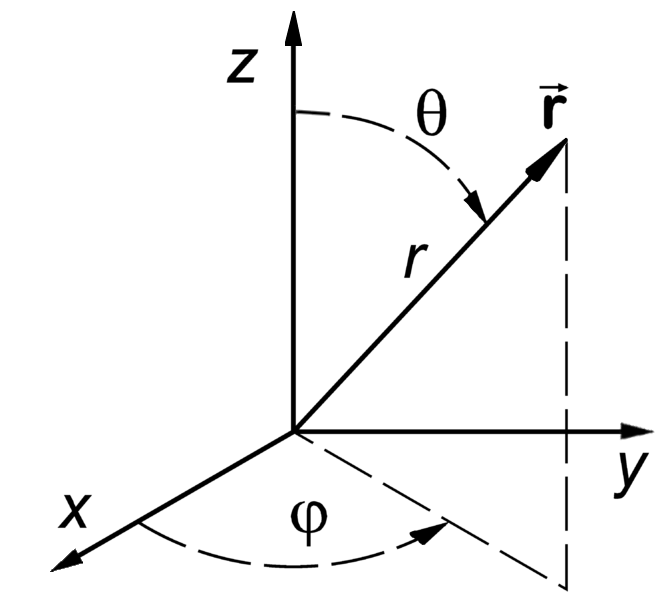
\includegraphics[width=4.5cm]{Bilder/coordinate.png}
	\end{center}
	\caption[Coordinate System of Belle II]{A sketch of the coordinate system of Belle II}
	\label{fig:CoordinateSysytem}
\end{figure}

A sketch of the coordinate system is shown in figure \ref{fig:CoordinateSysytem}. The origin of the coordinate system corresponds to the interaction region. For the Cartesian coordinate system: The $z$-axis points in the direction of the magnetic field. This is also the so-called forward direction. The $y$-axis points up to the upper part of the detector. The $x$-axis points along the radial direction of the accelerator. In figure \ref{fig:CoordinateSysytem} also the spherical coordinate system is shown. Here $\theta$ corresponds to the polar angle and $\phi$ to the azimuthal angle.\cite{DevelopVertex}

\section{Vertex detector}
\label{sec:vertexDet}

The vertex detectors (VXD) is able to make precise measurements of the tracks of particles close to the interaction region. This allows the reconstruction of decay-vertices of long-lived particles. For this it is very important to determine the distance and the spatial resolution of the first measured hit, and the effect of multiple scattering.


\begin{figure}[h!]
	\begin{center}
		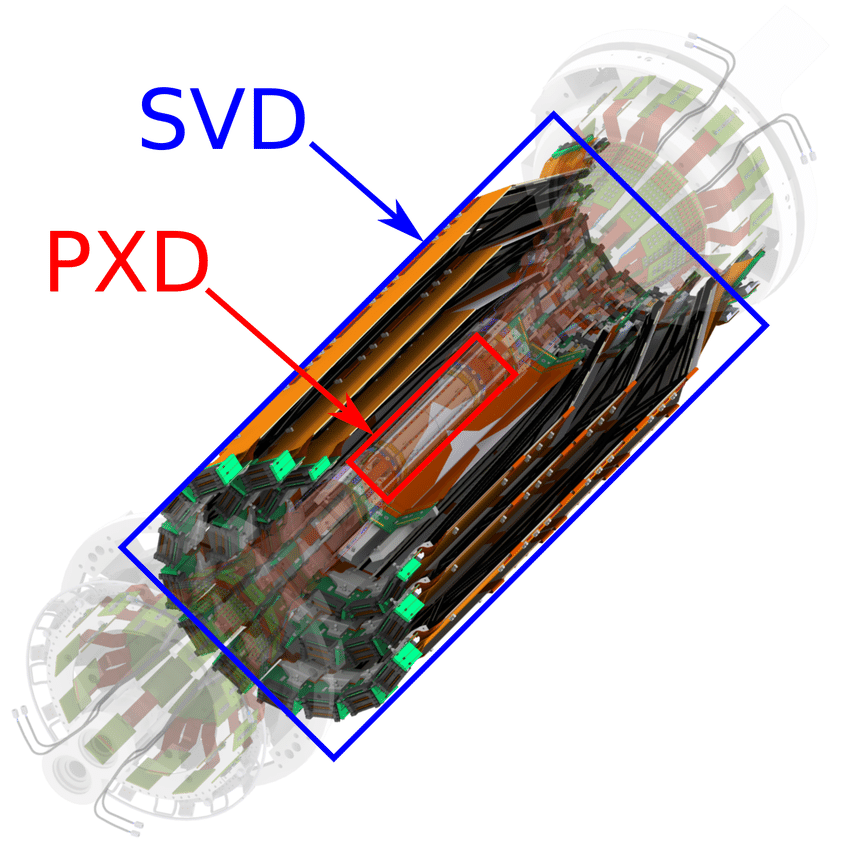
\includegraphics[width=10.5cm]{Bilder/PXD_SVD}
	\end{center}
\caption[Vertex Detector]{Sketch of the vertex detectors. The vertex detector itself consists of two sub-detectors. The PXD is surrounded by the SVD. \cite{OnlineDataReduction} }
\label{fig:VertexDet}
\end{figure}

The VXD consists of the pixel vertex detector and the silicon vertex detector, both can be seen in figure \ref{fig:VertexDet}. These two detectors complement each other.


\subsection{Pixel Vertex Detector}
\label{sec:Pixel}
The purpose of the PXD is to reconstruct the spatial position of the decay vertices of $B$, $D$ and $\tau$.
The PXD is based on Depleted P-channel Field-Effect Transistor (DePFET) technology. This technology allows the sensors of the PXD to be very thin ($50\,\mu\textrm{m}$).

\begin{figure}[h!]
	\begin{center}
		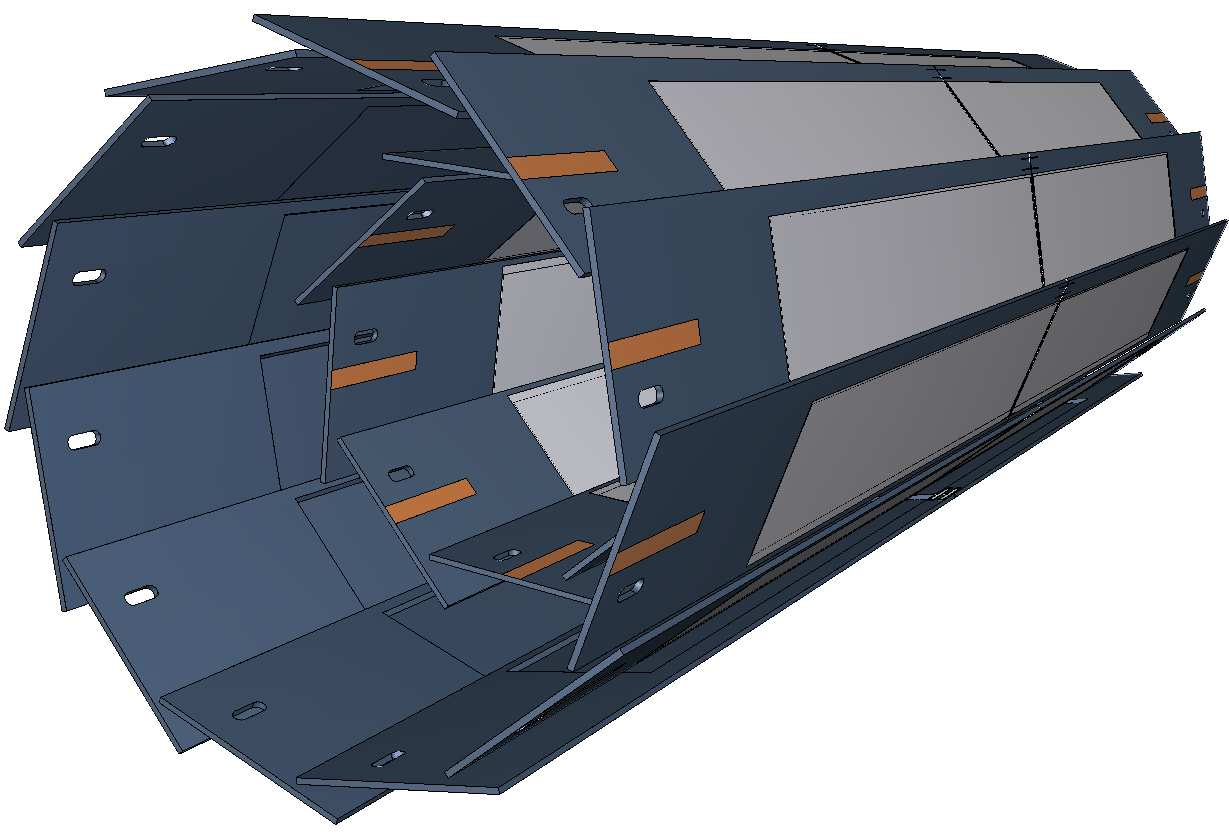
\includegraphics[width=10.5cm]{Bilder/pixel}
	\end{center}
	\caption[Pixel Detector]{Sketch of the PXD \cite{B2TR}}
	\label{fig:pxd}
\end{figure}

As you can see in figure \ref{fig:pxd}, the PXD consists of two layers of sensors. The inner layer is made out of eight planar sensors (ladder), each has a width of $15\,\textrm{mm}$ and an effective length of $90\,\textrm{mm}$. This layer has a radius of $14\,\textrm{mm}$. The second layer consists of 12 planar sensors. These sensors also have a width of $15\,\textrm{mm}$, but a length of $123\,\textrm{mm}$. The radius for the second layer is $22\,\textrm{mm}$. The PXD provides a spatial resolution of about $1.2\,\mu\textrm{m}$.\cite{B2TR}

Due to the vicinity of the PXD to the interaction region, the quantum-electrodynamics background is very high, so the sensors  must withstand high radiation. The DePFET technology fulfills this condition. \cite{B2TR} \cite{MARINAS201159}
\newline 

DePFET is a semiconductor detector concept invented in 1987 by J. Kemmer and G. Lutz of the MPI for Physics. This concepts combines detection and amplification in one single device. \cite{B2TR}

\begin{figure}[h!]
	\begin{center}
		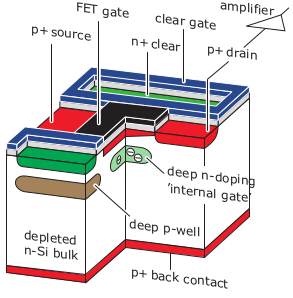
\includegraphics[width=7cm]{Bilder/DEPFET}
	\end{center}
\caption[DePFET]{Illustration of the DePFET technology.\cite{B2TR}}
\label{fig:DePFET}
\end{figure}

A cross section of the device is shown in figure \ref{fig:DePFET}. The structure of a DePFET cell consists of fully depleted silicon. In this silicon substrate depleted by a high negative voltage a $p-$channel MOSFET (metal oxide semiconductor field effect transistor) of a JFET (junction field effect transistor) is integrated. The field effect transistors act as a first pre-intensification. When radiation or a particle hists the detector, electron-hole pairs are created. These pairs get separated by the potential field of the sideward depletion. The positive charged holes drift to the negatively charged back contact. The negative charged electrons are collected in the potential minimum. The so-called internal gate. Above the internal gate a field emission transistor is located. The signal charged is amplified right above the position where it was generated. This avoids the leakage of lateral charge transfers. One of the most important main features of the DePFET is that the internal gate has a very small capacitance. This makes it possible to measure events affected by low noise even at room temperature.\cite{B2TR}

\subsection{Silicon Vertex Detector}
\label{sec:Silicon}

The SVD consists of four layers of double-sided strip detectors. The layers are located at radii of 38, 80, 115 and 140$\,\textrm{mm}$. There are two different shapes of these sensors. The rectangular sensors are used in the barrel part and the trapezoidal sensors are used in the forward region of the SVD. Each sensor has a thickness of $320\,\mu\textrm{m}$ but the sensors have different dimensions depending on the layer they are located. The barrel sensors in the most inner layer of the SVD have a dimension of $38.4 \times 122.8\,\textrm{mm}^2$. The size for the barrel sensors of the other layers is $57.6 \times 122.8\,\textrm{mm}^2$. The trapezoidal sensors have a dimension of $38.4\,\textrm{mm}$ on the small side of the trapez to $57.6\,\textrm{mm}$ on the long side of the trapez times a length of $122.8\,\textrm{mm}$.\cite{B2TR} An illustration of the SVD can be seen in figure \ref{fig:SiliconVertex}. 

\begin{figure}[h!]
	\centering
	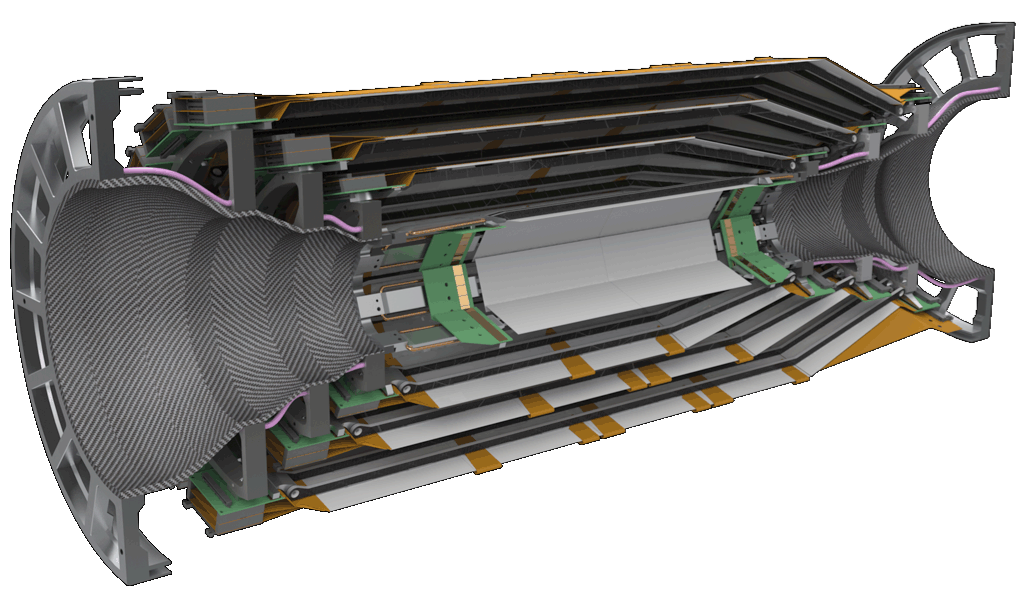
\includegraphics[width=12.5cm]{Bilder/SVD.png}
	\caption[Silicon Vertex Detector]{Cross section of the silicon vertex detector\cite{SVDItalian}}
	\label{fig:SiliconVertex}
\end{figure}

In the barrel region the $p$-side of the double-sided-strip sensors is arranged parallel to the beam axis and facing the interaction region. The $n$-side is facing outside the detector and the $n$-strips are perpendicular arranged to the beam axis. 

When a particles travels through the sensors it creates electron-holes pairs along its path by ionization. The electrons then propagate to the $n$-strips and are accumulated there. The holes propagate to the $p$-strips and are collected there. The sensors then produce a signal from which the coordinate of the particle position can be read out. The $p$-side provides the $z$-direction and the $n$-side provides the $r-\theta$ direction.\cite{B2TR} \cite{bergauer2010silicon}



\section{Central Drift Chamber}
\label{sec:CDC}

The CDC surrounds the SVD. It consists of 14336 wires arranged in 56 layers and has an inner radius of $16\,\textrm{cm}$ and an outer radius of $113\,\textrm{cm}$. The volume is filled with a $50\%\,\textrm{helium}$ and an $50\%\,\textrm{ethane}$ gas mixture. The purpose of the CDC is to reconstruct the momenta and tracks of charged particles, to identify these particles by measuring their specific energy loss within the gas volume. The CDC alone is able to identify low-momentum tracks, which are unable to reach the particle identification device. The CDC also acts as a reliable trigger for charged particles.\cite{B2TR} A small cross section of the CDC is shown in figure \ref{fig:CDC}.

\begin{figure}[h!] 
	\centering
	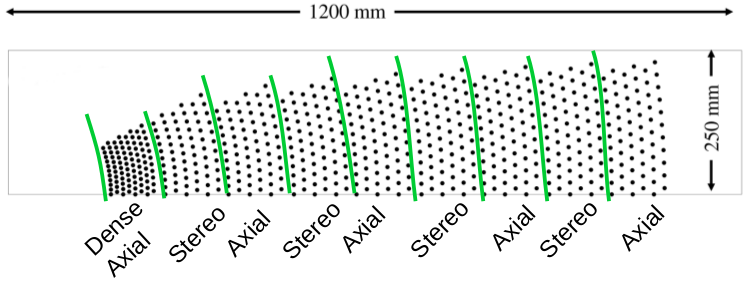
\includegraphics[width=12.5cm]{Bilder/CDC}
	\caption[Central Drift Chamber]{Cross section and only a small part of the CDC. Each dot represent a wire. Also the area for the different superlayers is shown by the green line. All of these wires are immersed in a helium-ethane mixture.\cite{CDCHauth}}
	\label{fig:CDC}
\end{figure}

When a charged particle passes trough the CDC it losses energy due to ionization of the gas. This produces electron-ion pairs, which are then separated by the electric field provided by 42240 aluminum field wires, with a diameter of $125\,\mu\textrm{m}$. The signal is then read out by the sense wires. These have a radius of $30\,\mu\textrm{m}$ and are made out of gold-plated tungsten.\cite{B2TR} 

As indicated in figure \ref{fig:CDC} there are different superlayers in the CDC. The Dense Axial and Axial sense wires allow the reconstruction of the track in the $r-\phi$ plane. The stereo sense wires gives information about the $z$ direction. These stereo wires are tilted in respect to the $z$ direction. Six layers of sense wires are combined to a superlayer. The CDC consists of five axial superlayers (A),and four stereo superlayer. The four stereo superlayer subdivide into two stereo superlayer (U) with a positive stereo angle and two stereo superlayers (V) with a negative stereo angle. Starting with the innermost superlayer, every second superlayer is an axial superlayer. The stereo superlayers are between them, alternating between U and V. In total there are nine superlayers. The innermost superlayer is called \textit{small-cell chamber} has a total of eight superlayers. (compared to the other superlayers with just six layers) This was done to lower the influence of the background, which is higher in the innermost superlayer due to the vicinity to the interaction region.
The CDC has a spatial resolution of about $100\,\mu\textrm{m}$.\cite{B2TR}

\section{TOP and ARICH}
\label{sec:ARTO}

There are two additional detectors for particle identification, the TOP and the ARICH. The TOP counter is located in the barrel part and it uses a combination of time-of-flight and Cerenkov angle measurements.
When a charged particle with the velocity $\beta$ is faster than the speed of light $c_n$ in a medium  with a reflective index $n$ then this particle emits Cerenkov radiation under the angle $\theta_{C} $.\cite{cerenkovAngle}


\begin{equation}
c_n = \frac{c_0}{n} \leq \beta	
\end{equation}

The Cerenkov angle is given by:\cite{cerenkovAngle}

\begin{equation}
\textrm{cos}(\theta_C)=\frac{1}{n\beta}
\end{equation}

\begin{figure}[h!]
	\centering
	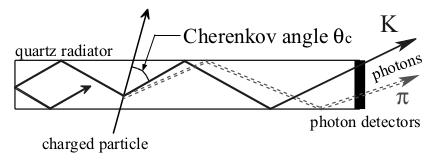
\includegraphics[width=10.5cm]{Bilder/TOP}
	\caption[TOP Principle]{Operating mode of a TOP detector.\cite{B2TR}}
	\label{fig:TOP}
\end{figure}

Figure \ref{fig:TOP} shows an illustration of the functionality of a TOP bar. The charged particle emits Cerenkov light when it passes the quartz crystal. These photons then travel inside the crystal due to reflection until they are detected by a photon detector. Measuring the time difference between the emitted photons it is possible to calculate the position of the track of the charged particle. The outgoing photons are then focused by mirrors and are then detected by PMTs. Cerenkov photons with different $\theta_C$ will be detected by different PMTs. Therefore, the TOP reconstruct the Cerenkov ring image using the information of time, $x$ and $y$.\cite{B2TR} 

The TOP counter consists of 32 quartz bars. They have a length of $1250\,\textrm{mm}$, a width of $45\,\textrm{mm}$ and a depth of $20\,\textrm{mm}$. There are two quartz bars per module. The TOP counter has a $K/\pi$ separation of over $99\,\%$.\cite{B2TR}

The ARICH detector is located in the forward endcap region. It is designed to distinguish between kaons and pions over most of their momentum spectrum. It is also able to identify particles with a momentum below $1\,\textrm{GeV}$.

\begin{figure}[h!]
	\centering
\begin{minipage}[b]{0.45\linewidth}
	\centering
	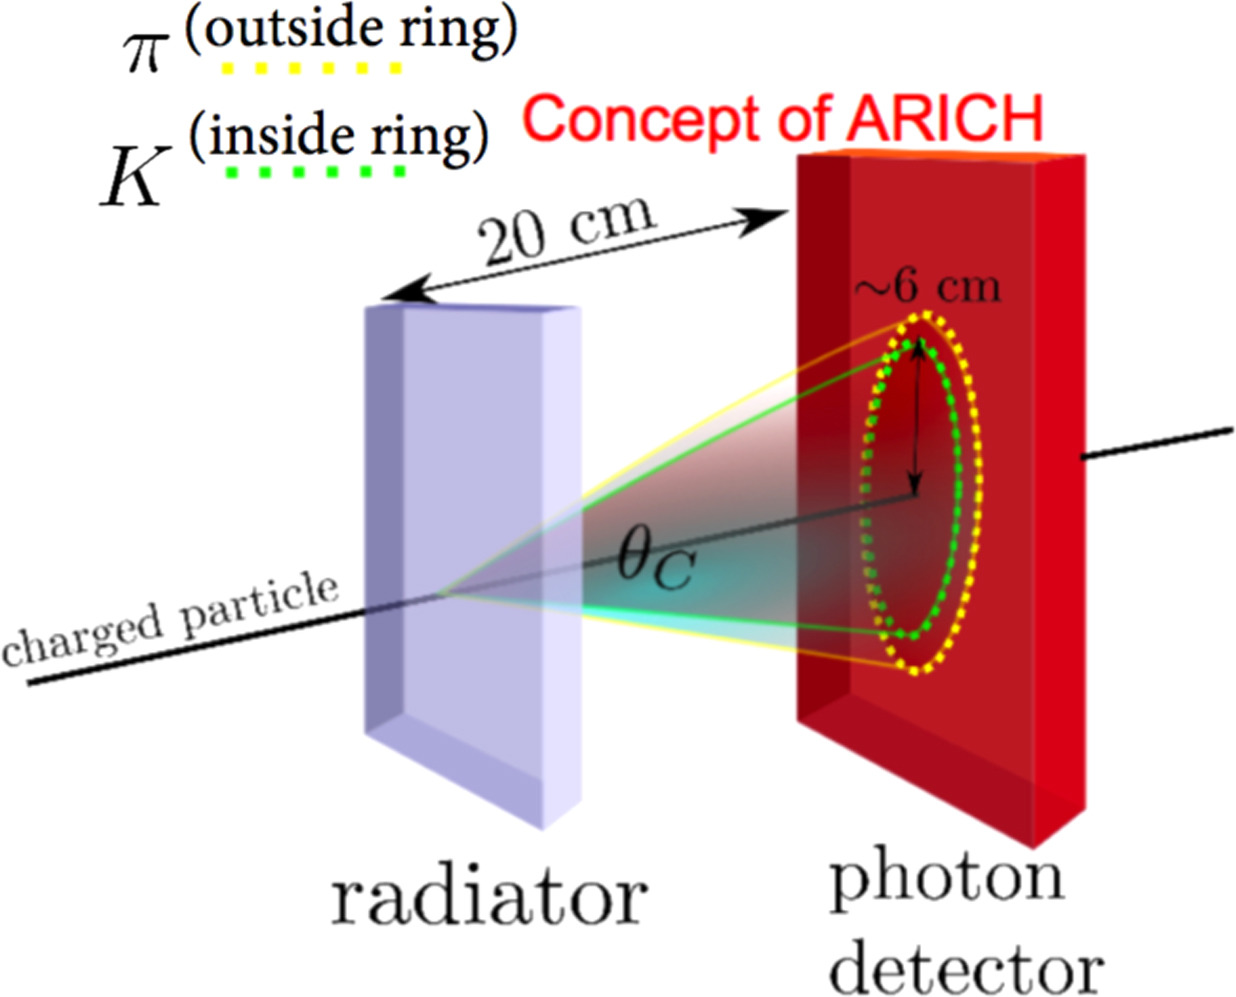
\includegraphics[width=\textwidth]{Bilder/ARICH}
\end{minipage}
\hspace{0.5cm}
\begin{minipage}[b]{0.45\linewidth}
	\centering
	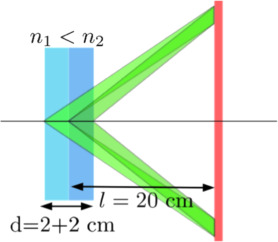
\includegraphics[width=\textwidth]{Bilder/ARICH2}
\end{minipage}

	\caption[ARICH]{Left: Illustration of the working principle of the ARICH detector. The yellow Cerenkov ring on the photon detector is produced by a $\pi$, the green ring by a $K$. Right: The radiator is shown in more detail. The radiator consists of two aerogel layers with different reflective index. \cite{TORASSA} }
\label{fig:ARICH}
\end{figure}

In figure \ref{fig:ARICH} the working principle of the ARICH detector is shown. A charged particle passes through two layers of an aerogel radiator with different reflective indexes and emits Cerenkov photons under an Cerenkov angle $\theta_C$. Behind the radiator is an extension volume for the Cerenkov rings to form. At a distance of $20\,\textrm{cm}$ behind the radiator is the photon detector.\cite{B2TR} Once the Cerenkov ring is reconstructed, the radius of the ring can be determined and, knowing the distance and the radius, the Cerenkov angle can be calculated.

\section{Electromagnetic Calorimeter}
\label{sec:ECL}

One of the main tasks of the ECL is the detection of photons with a high efficiency. It also determents the energy and the angular coordinates of these photons with high precision. It is also used for electron identification and the generation of a proper signal for the trigger. The ECL consists of a $3\,\textrm{m}$ long barrel section with an inner radius of $1.25\,\textrm{m}$. The circular endcaps are located at a distance of $z=1.96\,\textrm{m}$ in the forward direction and $z=-1.02\,\textrm{m}$ in the backward direction from the interaction point. The ECL covers a polar angle region of $12.4^{\circ} < \theta < 155.1^{\circ}$. Due to construction, there are two $ \sim 1^{\circ}$ wide gaps between the barrel and the endcaps. The barrel section of the calorimeter consists of 6624 CsI(Tl)\footnote{Thallium activated Cesium Iodide} crystals with 29 distinct shapes. Each of these crystals is a truncated pyramid with an average size of about $6\times6 \, \textrm{cm}^2$ in cross section and $30\,\textrm{cm}$ in length. The length of these crystals corresponds to around 16.1 radiation lengths $X_0$. The endcaps consist of 2122 CsI crystals of 69 shapes. At the end of each crystal, photo-multiplier are mounted to detect the excitation of the scintillators. The detected number of photons corresponds directly to the energy released by absorbed particles.
The energy resolution of the calorimeter can be approximated as:\cite{B2TR} \cite{Belle_ECL_2015}

\begin{equation}
\frac{\sigma_E}{E} = \sqrt{\bigg(\frac{0.066\%}{E}\bigg)^2 + \bigg(\frac{0.81\%}{\sqrt[4]{E}}\bigg)^2 + (1.34\%)^2}
\end{equation}
The energy E is in GeV.
\newline

Photons and electromagnetic particles are creating electromagnetic cascades when they pass through material.\cite{leo2012techniques} When a high energetic photon passes through a material it creates an electron-positron pair by pair production. For this, the photon must have at least an energy of $2\cdot m_{e^{-}} = 1.022\,\textrm{MeV}$. This energy is evenly distributed between the two particles. Because these two particles are charged and their velocity changes in an the electric field of a nuclei, they generate photons through Bremsstrahlung. These processes are repeated and a electromagnetic shower is created. The energies of the particles continue to decrease until the critical energy $E_c$ is reached. At the critical energy, the energy loss due to Bremsstrahlung is as high as the energy loss due to ionization.

If the average energy of an electron becomes ${E_0}/{e}$ then the distance the electron traveled is called radiation length $X_0$.

Assuming that the electromagnetic particles and photons interact after one radiation length and that they loose half of their energy each time they do, the total number of particles and their energy after $t$ cascades can then be calculated by:\cite{leo2012techniques}

\begin{equation}
	N \simeq 2^t
\end{equation}

\begin{equation}
	E(t) \simeq \frac{E_0}{2^t}
\end{equation}

This shower both spreads longitudinally and transversely. The transverse propagation can be described by the Moli\`ere radius. It can be calculated by:

\begin{equation}
	R_M=21\,\textrm{MeV}\cdot \frac{X_0}{E_c}
\end{equation}

$ 95\,\%$ of all particles of a shower are within two Moli\`ere radii.\cite{leo2012techniques}

\section{$K_L^0$ and muon detector }
\label{sec:KM}

The KLM consists of an alternating sandwich structure of a $4.7\,\textrm{cm}$ thick iron plates and resistive plate chambers (RPC) in between.

RPCs consist of two glass sheets, separated by a thin gas volume. These sheets act as high voltage electrodes. When a particle passes through the volume, they create ion-electron pairs which are then accelerated by the strong electric field. They therefore initiate more ionizations, which leads to a streamer between the electrodes. This causes a voltage drop in the nearby electrodes, which is detected by pick-up strips, located on both sides of the chamber. These strips are a few centimeters wide and are placed orthogonal on each side. Therefore, the particle track can be localized in $z/\phi$ for the barrel region and $\phi/\theta$ for the endcaps.

To distinguish between muons and hadrons, the KLM takes advantage of the high penetration power of muons. Hadrons deplete their energy through hadronic showers in the ECL and KLM. Electrons have a shorter radiation length and are therefore absorbed by the ECL, most of the time. $K_L^0$ create clusters in the ECL and the KLM. These clusters are than grouped and geometrically matched to charged tracks which are detected by the inner detectors. If no corresponding charged track can be found by geometrical matching, the detected particle is then treated as $K_L^0$ candidate.\cite{B2TR}\cite{KLMS}

\chapter{Trigger and Data Acquisition System}
\label{sec:TDAS}


\chapter{Tools}
\label{sec:Tools}




\section{Root}

Entsprechend kann es bei einer theoretischen Arbeit sinnvoll sein,
die L\"osungsmethoden in einem eigenen Kapitel zu beschreiben.

\section{Basf2}

Hauptteil Ihrer Arbeit ist das Kapitel (oder die Kapitel) mit den 
Ergebnissen. Bei einer theoretischen Arbeit kann damit auch 
die Herleitung von Formeln oder die Beschreibung eines Computerprogramms 
gemeint sein.

\chapter{Tracking Efficiencies}
\label{sec:TrackingEff}

In this chapter the tracking efficiency studies I did will be presented. I will go through my studies in more or less chronological order, from the reproduction of Sam Cunliffs plots to the calculation of different efficiencies.



\section{Definition of Efficiency}
\label{sec:Eff}

First of all, a definition of efficiency has to be declared, since there are different ways to define a tracking efficiency. The physics case I am considering is Bhabha events $ \textrm{e}^+ \textrm{e}^- \rightarrow \textrm{e}^+ \textrm{e}^- $. As described in chapter \ref{sec:SetupKEK}, charged particles leave a track in the detector. So, when we look at a outgoing particle with a track, then we know that the other particle should also have a track. If the other particle has no charge, then this is an inefficiency. If both particles have a track associated, then this is the efficient case.

So for this work I use the following definition of efficiency:

\begin{equation}
	\epsilon = \frac{\textrm{Number of Bhabha events with exactly 2 tracks}}{\textrm{Number of Bhabha events with 1 or more tracks}}
	\label{eq:efficiency}
\end{equation}

d



\section{Reproducing Sam Cunliffs Plots}
\label{sec:repSam}


\begin{figure}[h!]
	\centering
	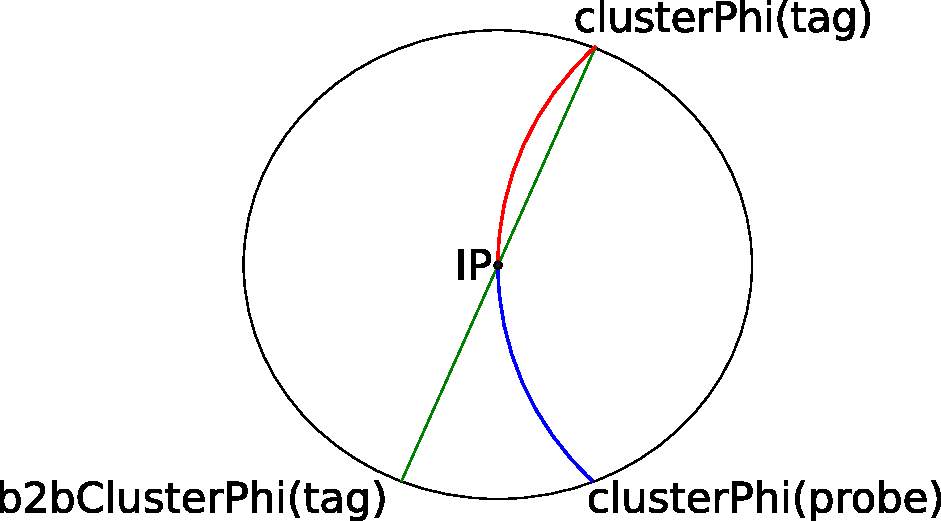
\includegraphics[width=10cm]{Bilder/b2b_2}
	\caption[Sketch of the b2b methode]{Created with Inkscape}
	\label{fig:Sketchb2b}
\end{figure}


%_______________________________________________________________________________
\chapter{Zusammenfassung und Ausblick}

In der Zusammenfassung sollten Sie in knapper Form die Aufgabenstellung 
und die wichtigsten Ergebnisse rekapitulieren. Es ist f\"ur die 
Gutachter hilfreich, wenn Sie ausdr\"ucklich beschreiben, worin 
Ihre eigenen Beitr\"age liegen. Scheuen Sie sich auch nicht davor 
auszusprechen, welche Untersuchungen durch die Zeitbegrenzung der 
Bachelorarbeit nicht m\"oglich waren und nutzen Sie dies als 
\"Uberleitung zu einem Ausblick auf m\"ogliche weitergehende 
Arbeiten an der Aufgabenstellung.

%_______________________________________________________________________________
\begin{appendix}
\chapter{Appendix}

\section{Tabellen und Abbildungen}

In der Regel sind die in Tabellen und Abbildungen enthalten Informationen 
so wichtig, dass sie im Hauptteil der Arbeit erscheinen sollten. Unter 
Umst\"anden sind aber erg\"anzende Tabellen und Abbildungen gut in einem 
Anhang aufgehoben. Wie im Hauptteil sollten Sie auch hier darauf achten, 
dass die in Tabellen und Figuren (siehe Abb.\ \ref{Abb:1}) dargestellte 
Information im Text angesprochen wird und selbsterkl\"arende Legenden 
vorhanden sind.
\medskip


%_______________________________________________________________________________
\section{Weiterf\"uhrende Details zur Arbeit}

Manch wichtiger Teil Ihrer tats\"achlichen Arbeit ist zu technisch 
und w\"urde den Hauptteil des Textes un\"ubersichtlich machen, 
beispielsweise wenn es um die Details des Versuchsaufbaus in einer 
experimentellen Arbeit oder um den f\"ur eine numerische Auswertung 
verwendeten Algorithmus geht. Dennoch ist es sinnvoll, entsprechende 
Beschreibungen in einem Anhang Ihrer Bachelorarbeit aufzunehmen. 
Insbesondere f\"ur zuk\"unftige Arbeiten, die an Ihre Bachelorarbeit 
anschlie{\ss}en, sind dies manchmal hilfreiche Informationen.

%_______________________________________________________________________________
\listoffigures
\listoftables
%\chapter{Bibliography}

Machen Sie genaue Angaben, so dass die verwendeten Literaturstellen 
eindeutig identifiziert und aufgefunden werden k\"onnen.
Bei Lehrb\"uchern ist es sinnvoll, 
den Titel anzugeben, eventuell auch die Ausgabe. Bei Artikeln in 
Fachzeitschriften ist es \"ublich, nur die 
gebr\"auchlichen Abk\"urzungen f\"ur den Titel der Zeitschrift, Band, 
Erscheinungsjahr und Seite anzugeben. Unter Umst\"anden kann es auch 
sinnvoll sein, im Internet aufgefundene Informationsquellen anzugeben, 
zum Beispiel f\"ur Software oder zu den Details von 
Ergebnissen gro{\ss}er experimenteller Kollaborationen. Es ist 
selbstverst\"andlich, dass Sie auch Bachelor, 
Diplom- oder Doktorarbeiten angeben, wenn Sie diese in Ihrer eigenen 
Arbeit verwendet haben.
\medskip

Im folgenden Beispiel werden die in der Datei %{\tt h-physrev3.bst} 
enthaltenen Anweisungen als Stilvorlage verwendet. Andere 
M\"oglichkeiten f\"ur die Gestaltung eines Literaturverzeichnisses 
findet man im Internet: \url{http://janeden.net/bibliographien-mit-latex}.


\nocite{*}
\printbibliography[title={Bibliography}]


%_______________________________________________________________________________
\chapter{Danksagung}

... an wen auch immer. Denken Sie an Ihre Freundinnen und Freunde, 
Familie, Lehrer, Berater und Kollegen.

\end{appendix}

\end{document}  
        
        